\section{What inspection saves on held-out data (Member~4)}
\label{sec:m4}
\textbf{Code:} \code{experiments/task5\_inspection.py}.

The last step returned to the predictions of the exact model in Section~\ref{sec:m6} and checked them
with fitted models. For each of the 20 splits the experiment draws $10{,}000$ emails from that
one-dimensional model and uses the standard Spambase split (standardised features). It fits the shared
Gaussian model and logistic regression, tuned on validation log-loss, and applies three rules to the
same test probabilities: the accuracy cut $0.5$, the cost cut $10/11$, and the rule with inspection at
a range of prices $\ci$.

\begin{table}[!htbp]
\centering\small
\input{\resultsdir/c6_rules.tex}
\caption{Accuracy and cost per email of the two automatic rules on test data
(mean $\pm$ standard error, 20 splits, $\cfp=10$, $\cfn=1$).}
\label{tab:c6-rules}
\end{table}

\begin{table}[!htbp]
\centering\small
\input{\resultsdir/c6_savings.tex}
\caption{Inspection at $\ci=0.3$: cost of the best automatic rule, cost with inspection, the paired
saving and the share of emails inspected.}
\label{tab:c6-savings}
\end{table}

\begin{itemize}
  \item \emph{More accurate means more expensive.} Moving the cut from $0.5$ to $10/11$ lowers the
        Gaussian model's synthetic accuracy from $84.6\%$ to $73.9\%$ and cuts its cost from $0.780$ to
        $0.309$ (Table~\ref{tab:c6-rules}). Both models show the same ordering on Spambase.
  \item \emph{The fitted models match the exact model.} At $\ci=0.3$ it predicts a cost of $0.179$
        with $41.6\%$ inspected; the fitted Gaussian model gives $0.181$ and $41.7\%$, and the curves
        agree at every price (Figure~\ref{fig:c6-syn}).
  \item \emph{Inspection pays on real data.} On Spambase, logistic regression saves $0.100$ per email
        by inspecting $24.1\%$ of them, and the Gaussian model saves $0.121$ (Table~\ref{tab:c6-savings}).
        Figure~\ref{fig:c6} shows that the saving shrinks as inspection gets dearer and vanishes at
        $\ci=10/11$, where both models stop inspecting.
  \item \emph{Not an artefact of duplicates.} $9.8\%$ of Spambase test rows also appear in their
        training split. Without them inspection still cuts the cost from $0.264$ to $0.160$ (logistic)
        and from $0.291$ to $0.173$ (Gaussian).
\end{itemize}

\begin{figure}[!htbp]
\centering
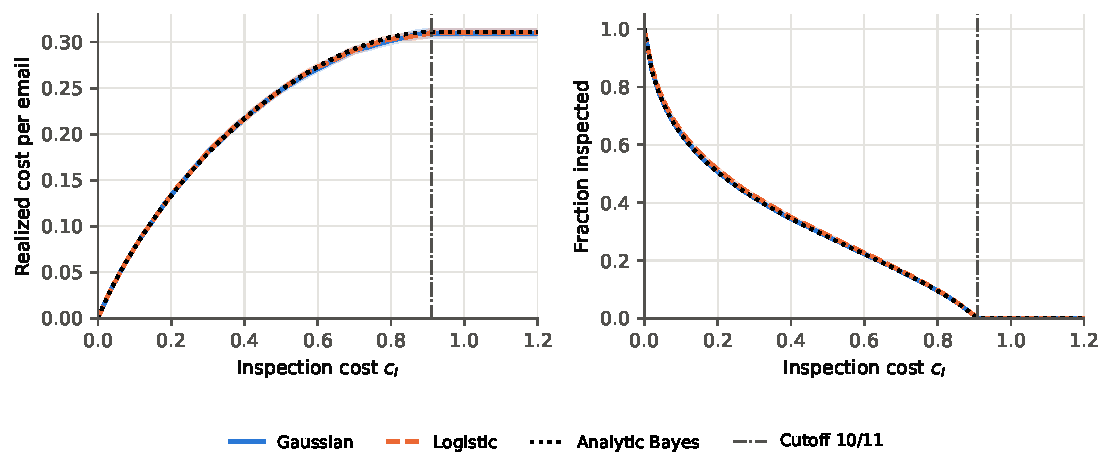
\includegraphics[width=0.92\linewidth]{c6_inspection_synthetic.pdf}
\caption{Synthetic data: test cost (left) and share inspected (right) of the fitted models against
$\ci$, with the exact values for the true posterior. The lines overlap.}
\label{fig:c6-syn}
\end{figure}

\begin{figure}[!htbp]
\centering
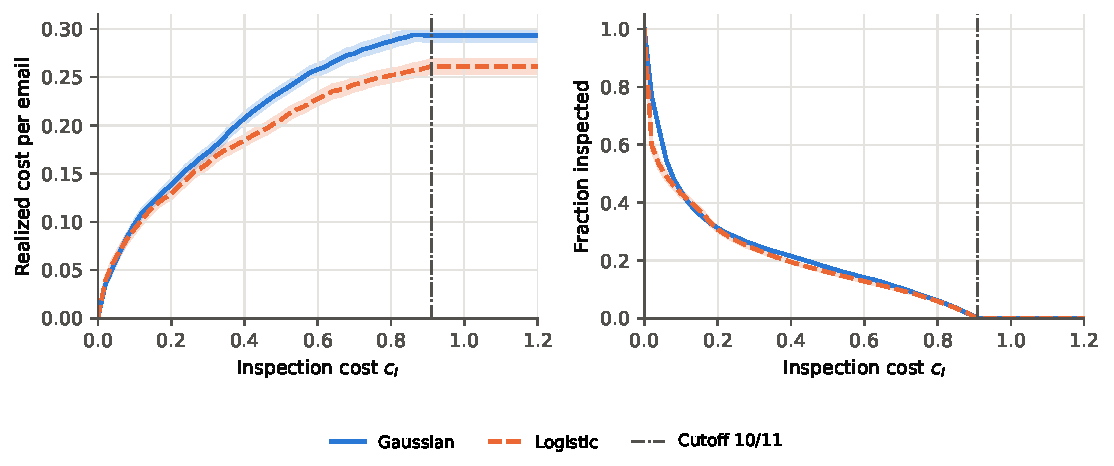
\includegraphics[width=0.92\linewidth]{c6_inspection_spambase.pdf}
\caption{Spambase: test cost (left) and share of emails inspected (right) against the inspection
price $\ci$ (bands: $\pm1$ standard error). The vertical line marks $\cstar=10/11$.}
\label{fig:c6}
\end{figure}
